\chapter{Temporal Property Detection with Numerical Dependencies and
Resampling}\label{chap:tempresult}

We now present our temporal logic for knowledge discovery applied to
real world data. In section~\ref{sec:tr_intro} we discuss  the context
of our experiments and present the model for the discovery of
properties in section~\ref{sec:tr_propmodel}. The model we provide,
given the flexibility of our logic, is not rigid and numerous
algorithms may be created to extend or diverge from this model. 
We present one algorithm in this context, noting that other algorithms
are direct implementations of the semantics provided by the logic. 
The results of our
experiments are presented in two sections. Firstly,
in~\ref{sec:tr_relseq} we present results gained from temporal
relation sequences satisfying NDs. Then, in
section~\ref{sec:tr_tsares} we discuss results from experiments on
standard time series data obtained from financial stocks. We present
an analysis or our work in the context of this research area in
section~\ref{sec:tr_analysis}. Real-world applications
of both our logic and the model in which to
apply it are given in~\ref{sec:tr_realworld}.
We conclude in section~\ref{sec:tr_disc}.

\section{Introduction}\label{sec:tr_intro}

The flexibility of the
logic implies that the knowledge discovery process requires
restriction of the types of rules found to prevent trivial rules being
discovered; we therefore focus on response and persistence properties
for pairs of temporal datasets. The discovery of properties expressed with
the temporal connectives defined here has not previously been
used. Obviously our 
work is closely related to other work on rule discovery though our
logic allows for temporal relationships to be discovered. As we have
seen in~\ref{subsec:temp_mine}, \cite{bt98} is
a recent work which uses temporal logic for rule discovery; the logic
used is a standard temporal logic and as such requires restriction for
interesting patterns to be found. The use of properties places such a
restriction on patterns to be discovered whilst at the same time
ensures interesting discovery.

\medskip


Our property discovery model incorporates aspects of the property
classification hierarchy thereby simplifying the knowledge discovery
process. We move from obtaining values of statistical functions at the
sequence level to the creation of safety and guarantee rules and then
to a larger sequence size for the discovery of more complex
properties, such as response and persistence.
Within the knowledge discovery process we employ moving blocks
resampling to discover short range properties. The moving blocks
bootstrap considers all possible blocks of a given size $n$ within an
input time series. A resampled time series is then formed by randomly
selecting blocks from the original series and appending each block to
the resampled series until the resample is equal to or greater than
the length of the original series.  Different time series are sampled
from simultaneously so that relationships between series are preserved
within blocks. Property discovery may then be
applied to this resampled sequence knowing that relationships have
only been preserved within blocks. We show that useful conclusions can
be found from this process, particularly in conjunction with property
discovery from the original process.

\medskip

We applied our property discovery model to a number of different data
sets including National Football League (NFL) data over 3 seasons and data
sets of US National Notifiable disease data, both of which we could
mine for ND set satisfaction. Restricting our logic solely for time
series we then applied our methods to stocks from the FTSE 100. We found
rules which complement the graphical depiction of a time series. To
illustrate, we found the following property in two oil stocks, BP ($bp$) and
SHELL ($sh$), represented as \pers{30}{15} ($bp$ $\downarrow_r$ $v_1$
$\wedge^0$ $sh$ $\downarrow_r$ $v_2$) where $\downarrow_r$ implies a downward
regressive trend and $v_1,v_2$ are the initial values of the stock
when the rule holds (found at 7 locations over 242 days).  Graphical analysis of these stocks would suggest
a similar upward relation but this was not found for these sequence
sizes suggesting downward trends have lasted longer than upward from 1
December 1997 to 1 November 1998 for these stocks. Many additional results 
showed that interesting and unexpected properties were
discovered which we detail and analyse, which both complemented and
extended a graphical depiction.

\medskip

For the sake of clarity we often present rules without specific values
which we believe would not aid in the presentation or understanding of
the rule.

\section{Property Discovery Model}\label{sec:tr_propmodel}
\index{Temporal Properties}



\begin{figure}[ht]
\centerline{\scalebox{0.6}{\includegraphics{../Event_theory/model2.eps}}}
\caption{\label{fig:model2} A description of our Temporal Property
Discovery System}
\end{figure}


We now describe our property discovery model presented in
Figure~\ref{fig:model2}. Input is a sequence of $n$ relation states.
Each relation in this sequence
satisfies a set of NDs. We wish to provide details of {\em properties}
which may hold in the sequence. From the initial relation sequence we
form series of moving averages of windows, each of size $w$ so that
the sequences we in effect deal with are
moving average sequences of the original relation sequences, each of
size $n - (w-1)$, to all for trend detection. 
We have the option of employing {\em Jackknife}
resampling \cite{efr82}, for smoothing, at this point so that the sequences are robust i.e. noisy
outliers are weakened by the use of resampling.  We consider examples both with
and without Jackknife resampling. We can also apply the moving blocks
bootstrap to recreate time series for short range property detection.
\medskip


Using
this information we then can gain trend, cross- and auto-correlation,
and sequence description information. We then examine for correlation
and sequence description purposes all sequences of a fixed size
$n$. This allows us to search for properties in a bottom up fashion with
regard to the sequence size $n$. For example, if we are looking for
safety property satisfaction we can examine all sequences of size
greater than $n$ until either we can go no further or the property is
satisfied. We propose obtaining an input for a larger size sequence
$m$ so
that properties are detected with respect to $m$ and $n$. Flexibility
is therefore obtained by looking for patterns of $n$ time points
within larger sequences $m$ time points. This gives us much additional
flexibility. This property discovery can occur in a combination of
bottom up or top down methods depending on the property we are looking
for.

\medskip

If all sequences of a
fixed size satisfy a rule we refer to this as a {\em seasonal property},
whereas if there exist a set of sequences such that a property holds
throughout the complete sequence but not for subsequences of a fixed
size, which we denote as a cover then this may imply irregular
behaviour. As we have shown it takes exponential time to search for
such properties.
If any of these properties occur not for the complete sequence we
may denote this by creating persistent (ordered/correlated)
properties.



\subsection{The Generic Property Discovery Algorithm}\label{subsec:tr_genalg}

In the data mining literature there has been much discussion of
working towards a common framework for data mining, presenting
comparisons of data mining now to database research in the 60s before
the adoption of the relational model \cite{fps96b,man96}. Generic algorithms for data
mining have been proposed, most notably by Manilla \cite{man96},
extended in \cite{man97}. We now outline this generic procedure. A
candidate set of initial patterns is provided by the user. The
database (or data set) is then examined to see if these patterns occur
a sufficiently frequent number of times, in which case they are
classified as interesting. A new candidate set is generated from the
interesting patterns and the previous candidate set and the process is
repeated. This is continued until there are no new candidate elements
and the interesting set is returned as knowledge discovered. We can
see that our algorithm~\ref{alg:propmine} has a similar skeleton to
this generic procedure. Our procedure is general in that we consider
the satisfaction of a property to be interesting and the natural
classification of properties allows properties to be discovered using
the input relation sequence and the properties previously discovered. 

{\line
\begin{figure}[ht]
\begin{center}
\fbox{\begin{minipage}{16cm}
\begin{algorithm}[{\rm Property\_Mine}($\Delta$, F, $n$)]\label{alg:propmine}
\begin{rm}
\begin{tabbing}
t1\=t2\=t3\=t4\=t5\=t6\=t7\= \kill \\
\ra.  \> \> {\bf begin} \\
\sa.  \> \> \> Rule\_set :=  $\emptyset$; \\
\sa.  \> \> \> {\bf while} $\exists$ a new classifiaction of
properties {\bf do} \\
\sa.  \> \> \> \> {\bf for each} property $p$ at same classification $c$ {\bf do}\\
\sa.  \> \> \> \> \> Rule\_set := $p$ property discovered from
$\Delta$ and Rule\_set $\cup$ Rule\_set;\\
\sa.  \> \> \> \> {\bf end for}\\
\sa.  \> \> \> \> $c$ := Next classification of temporal properties \\
\sa.  \> \> \> {\bf end while }\\
\sa.  \> \> \> {\bf return} Rule\_set; \\
\sa. \> \> {\bf end.}
\end{tabbing}
\end{rm}
\end{algorithm}
\end{minipage}}
\caption{\label{tr:fig:propmine} The Generic Property Data Mining Algorithm}
\end{center}
\end{figure}
}



\subsection{The Response Persistence Algorithm}\label{subsec:tr_resppers}

In Algorithm~\ref{alg:resp}, detailed in figure~\ref{tr:fig:resp}, we
present a simple algorithm for detecting response and persistence
properties with respect to two sequence sizes given by the user. 

{\line
\begin{figure}[ht]
\begin{center}
\fbox{\begin{minipage}{16cm}
\begin{algorithm}[{\rm Response\_Persistence}($\Delta$, F, $n$, $m$)]\label{alg:resp}
\begin{rm}
\begin{tabbing}
t1\=t2\=t3\=t4\=t5\=t6\=t7\= \kill \\
\ra.  \> \> {\bf begin} \\
\sa.  \> \> \> Main\_Rule\_set :=  $\emptyset$; \\
\sa.  \> \> \> Final\_Rule\_set :=  $\emptyset$; \\
\sa.  \> \> \> {\bf for each} subsequence $s$ of $\Delta$ of size $m$ {\bf do}\\
\sa.  \> \> \> \> Rule\_set := $\emptyset$; \\ 
\sa.  \> \> \> \> Rule\_sequence := $\emptyset$; \\ 
\sa.  \> \> \> \> { \bf for each} subsequence $s_n$ of $s$ of size $n$
{\bf do}\\
\sa. \> \> \> \> \> Rule\_set$_{s_n}$ := Rule set discovered for $s_n$; \\
\sa. \> \> \> \> \> Rule\_sequence := Rule\_sequence $\leadsto$ Rule\_set$_{s_n}$; \\
\sa. \> \> \> \> \> Rule\_set := $\{$ Rule\_set$_{s_n}$ $\}$ $\cup$ Rule\_set; \\
\sa.  \> \> \> \> {\bf end for}\\
\sa.  \> \> \> \> M\_rule := $\emptyset$; \\
\sa.  \> \> \> \> M\_rule := $\{$ Rule\_sequence $\} \cup$ M\_rule; \\
\sa.  \> \> \> \> {\bf if } $\forall$ r $\in$ Rule\_set $\exists \sigma$
 such that $r \models \sigma$ {\bf then} \\
\sa.  \> \> \> \> \> M\_rule := $\{ \bm^n \sigma \} \cup$ M\_rule; \\
\sa.  \> \> \> \> {\bf end if};\\
\sa.  \> \> \> \> {\bf if } $\exists$ r $\in$ Rule\_set and $\exists r_2$
$\in$ Rule\_set with $r \not= r_2$ \\
\> \> \> \> \> such that $r \models \sigma$ and $r_2$
 $\not\models$ $\sigma$ {\bf then} \\
\sa.  \> \> \> \> \> M\_rule := $\{$ \diam$^n$ $\sigma \} \cup$ M\_rule;\\
\sa.  \> \> \> \> {\bf end if};\\
\sa.  \> \> \> \> Main\_Rule\_set :=  $\{$ M\_rule $\}$ $\cup$ Main\_Rule\_set; \\
\sa.  \> \> \> {\bf end for}\\
\sa.  \> \> \> {\bf if } $\forall$ r $\in$ Main\_Rule\_set $\exists \sigma$
such that r $\models \sigma$ {\bf then} \\
\sa.  \> \> \> \> Final\_Rule\_set := $\{ \bm^m \sigma  \} \cup$ Final\_Rule\_set; \\
\sa.  \> \> \> {\bf end if};\\
\sa.  \> \> \> {\bf if } $\exists$ r $\in$ Main\_Rule\_set and $\exists$ r$_2$
$\in$ Main\_Rule\_set with r $\not=$ r$_2$ \\ 
\> \> \> \> \> such that r $\models \sigma$ and r$_2$
 $\not\models$ $\sigma$ {\bf then} \\
\sa.  \> \> \> \> Final\_Rule\_set := $\{$ \diam$^m$ $\sigma \} \cup$ Final\_Rule\_set;\\
\sa.  \> \> \> {\bf end if};\\

\sa.  \> \> \> {\bf return} Final\_Rule\_set; \\
\sa. \> \> {\bf end.}
\end{tabbing}
\end{rm}
\end{algorithm}
\end{minipage}}
\caption{\label{tr:fig:resp} The Response Persistence Algorithm}
\end{center}
\end{figure}
}




\section{Relational Sequence Data Sets}\label{sec:tr_relseq}


We now discuss the experiments carried out and the results achieved
using NDLTL. Given the flexibility of our logic it is easy to extend
the results presented here by: 
\begin{itemize}
\item Allowing the user to query a given input. He may want to know,
using sales data obtained daily over 2 years, if there is a peak of sales in every quarter, and
express this using our logic. This example shows a possible
seasonality query which would take the form \resp{730}{90} (X
$\to^{\uparrow_r K}$ Y $\leadsto$ X
$\to^{\downarrow_r K}$ Y)
\item Modifying the time series functions within the logic. Different
functions can be incorporated, for example, that are specifically
known to handle nonlinear time series better than linear regression.
\end{itemize}

We now present the results, initially focusing on ND temporal relation
sequences and
then moving on to time series results alone. We focus on the latter
due to the lack of significant real-world data available for temporal
data (it is easier to obtain public data, such as share closing prices,
compared to a database of employee data over the last 20 years). We
also emphasise time series due to the availability of data with a
significant number of points, whereas a temporal database may only be
updated monthly/yearly, though this is changing for many automated
knowledge discovery and data warehousing applications.


\subsection{Results}\label{subsec:tr_relres}


We present two datasets used to obtain ND values, both publicly
available at Statlib, a data set resource (\ttb
http://lib.stat.cmu.edu\tte). The first we
discuss is (blind) records of disease data concerning occurrences of
mumps in the US from 1957 to 1989. These records contain the number of
patients for cases of mumps reported on a state-by-state
basis. Though we just obtained from the dataset the number of patients
per year suffering from mumps we note that this may have been
expressed in a database from where a relation was used for storing
patient data in the form of $\emptyset \to^k PATIENT\_ID$. We note
that when the left hand side of an ND is empty the branching factor of
the ND is a cardinality constraint on the domain size of the right
hand side attribute set. This is a small data set and we can see that
it has a downward trend in figure~\ref{graph:profb_1}. We use it for
illustration before moving on to more complex data sets. For the sake
of clarity we express both ND values such as $\emptyset \uparrow^k PATIENT\_ID$
simply as a marker of trend preceded by an identifier if the trends
are for different NDs or time series, e.g. $ohio\uparrow$. The
specific ND values are not important in this context particularly as
they are most probably related to population size which would need to
be normalised.
\medskip

The results obtained for a small sequence size of 5 years and a large
size of 10 years were \resp{10}{5} ($ohio\downarrow_r \wedge^0 alaska\downarrow_r$)
together with persistence results of the following form \pers{10}{5}
($ohio\downarrow_r \wedge^0 alaska\downarrow_r$). Clearly, these results tell us
that the number of cases in mumps is falling, continuously, without
significant fluctuation. For a comparison between the
number of cases in Alaska and Ohio we increased the sequence sizes to
12 and 20 and found, continuously throughout the sequence that the
following persistence rule holds: \pers{20}{12}
($ohio\downarrow_r \wedge^2 alaska\downarrow_r$). We see that the lag in
the downward trends (of 2 years) may provide an indication that the number of
cases falling is correlated with geographical regions. Obviously
expert knowledge is required to confirm this. 
Applying a simple pattern matching algorithm for comparing linear
trends within a sequence we find that \safe{12}
($\downarrow$,$\uparrow$, $\downarrow$) holds for Ohio. Therefore
although we have found the general trends to be downwards there are
peaks within larger sequences.

\smallskip
A complete description of the series is provided by ($ohio\downarrow_r
\wedge^1 alaska\downarrow_r$) $\leadsto$ ($ohio\downarrow_r
\wedge^2 alaska\downarrow_r$). We find the same rule from applying
discordance instead of linear regression. This rule concisely presents
the behaviour of the sequence. It is obtained from 12 year sequences
and compressed so that $\sigma \leadsto \sigma$ becomes $\sigma$. We
omit presentation of description rules for longer complex time series.
We can see from these simple results how properties of NDs over time
can be succinctly characterised within our logic. We now move on to a
slightly more interesting example.

\medskip

\begin{figure}
\centerline{\scalebox{0.6}{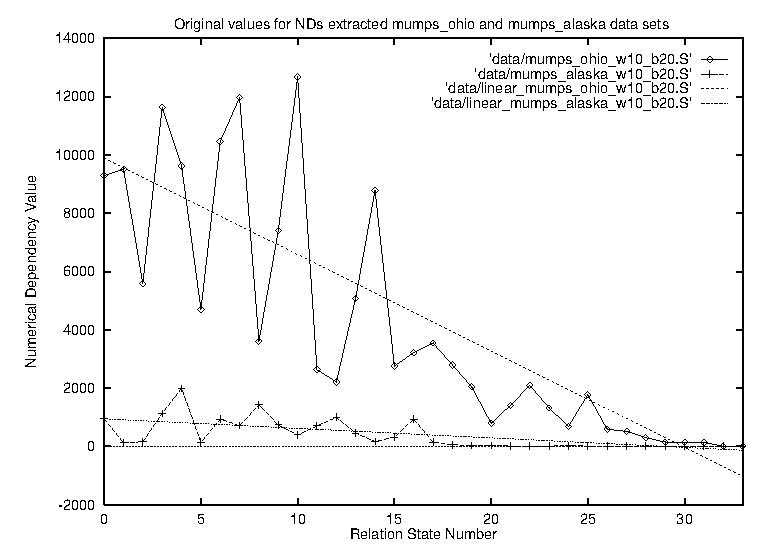
\includegraphics{../../CPP/Time/data/mumps_ohio_mumps_alaska.eps}}}
\caption{\label{graph:mumps_ohio_1}\scriptsize{Data values of Mumps
cases in Ohio and Alaska from 1957 - 1989}}
\end{figure}


\begin{figure}
\centerline{\scalebox{0.6}{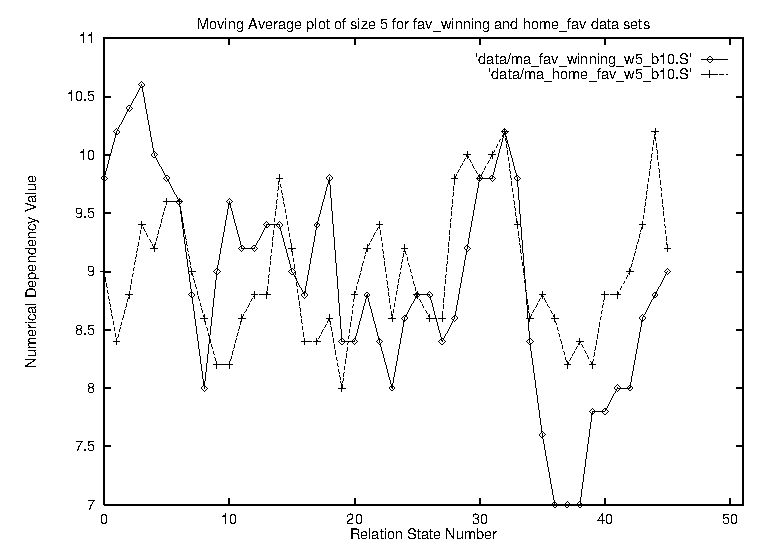
\includegraphics{../../CPP/Time/data/fav_winning_w5_b10data_ma.eps}}}
\caption{\label{graph:profb_1}\scriptsize{Data set values of two NDs
from NFL season data 1989-1991}}
\end{figure}



In Figure~\ref{graph:profb_1} we present the changing ND values for
two NDs obtained from relations containing Football Data. Each week of
the season, for three seasons from 1989 to 1991, details of team
results were stored in a database together with details of the
favourite team for each match. We obtained two NDs from the relation
$YEAR$ $WEEK$ $\to^k$ $FAV\_TEAM\_WIN$ and $YEAR$ $WEEK$ $\to^k$
$HOME\_FAV$. We note that each relation was contained $YEAR$ $WEEK$
$DAY$ representing the day the match was played on. Our figure shows
the two lines relating to changes in each ND. We can see no clear
trend in this figure for moving averaged data.

\medskip

For the two NDs we found the following property from the moving
average record of points with each moving average of size 5,
\pers{10}{5} ($HOME\_FAV$ $\uparrow_r \wedge^0$ $FAV\_TEAM\_WIN$ $\uparrow_r$) suggesting that an
increase in the home team winning is correlated with an increase in
the favourite team winning. This therefore expresses the fact
concisely and we can perhaps infer from this that the home teams are
most often the favourite team. Additionally, we examined the original
data set for patterns in sequences of 5 weeks and found none. It is
clear that the nature of the data contains no underlying trend.



\subsection{Resampling for Smoothing}\label{subsec:tr_res}
\index{Jackknife Resampling}
\index{Bootstrap Resampling}

\subsection{The Moving Blocks Bootstrap}\label{subsec:tr_mbb}
\index{Moving Blocks Bootstrap}


We introduce the Moving Blocks Bootstrap for verification of short
range event rules and provide details of its efficacy discussing the
results we found from its application.

\begin{definition}[Moving Blocks Bootstrap for Relations]
\begin{rm}
Given a relation sequence \linebreak[4] $\{ r_1, r_2, \ldots, r_N \}$
we construct blocks of relations where $MB_t$ is a block containing
$b$ relations such that $MB_t = \{ r_t, r_{t+1}, \ldots, r_{t+b-1} \}$
and there are $N - b+ 1$ blocks where $t = 1, 2, \ldots, N-b+1$. We
then resample $k$ moving blocks uniformly with replacement from $\{
MB_1, MB_2, \ldots, MB_{N-b+1} \}$ where $N \sim bk$. This may be repeated any number of times.
\end{rm}
\end{definition}

\smallskip

\centerline{\scalebox{0.7}{\includegraphics{../Event_theory/mbb.eps}}}
 
The moving blocks bootstrap forms an empirical distribution and this
distribution is the proposed bootstrap approximation. For a block
length $b$ all possible contiguous blocks of length $b$ within the
time series are available for selection. In \cite{et93} each moving
blocks bootstrap sample has an AR(1) model fitted to it to estimate
the parameter $\beta$. Results decreased upon an increase in the block
size, perhaps allowing us to infer that dependency was based on the
previous few points only (to any significant degree). The potential to
sample all possible contiguous blocks of a given size $b$ allows all
possible relationships of length less than or equal to $b$ to be sampled.



\section{Time Series Data Results}\label{sec:tr_tsares}



We now move on to examine more complex temporal data sets. We 
assume that the data is restricted to numerical data alone, although
if the data were stored in a suitable form in a database then NDs
might apply. When analysing time series we are not seeking to
discover what years of statistical analysis could not; indeed much of
this logic is based on statistical functions. Instead we are looking
for a concise representation that might convey specific properties
which hold at a certain time or throughout time and we express these
with our logic. The logic details properties in a machine
understandable form. 

\medskip

For the following study we focused on financial stocks from the FTSE
100. We analysed stocks in similar sectors seeing if there are general
properties from which we can infer information, concentrating on
financial, oil and retail sectors. We highlight some of the results
found and remark that all applications discovered possibly useful
properties. Our first analysis
focuses on BP and Shell. Under a story entitled ``bad times for the
oil industry'' in the Lex column of the Financial Times, November 4
1998, it was discussed how the oil industry has suffered in recent
months though some recent results (third quarter) posted by BP show
that a 35\% drop in profits is good news in comparison with a more
than 50\% drop by Shell prices. We can see from
figure~\ref{graph:bp_11mn_1} that BP ($bp$) has been outperforming
Shell ($sh$) in
terms of recent performance. We discovered however that the stocks are
related in short term performance, as we would expect. We found that
in Jan and Feb the following persistence property held \pers{90}{60}
($bp$ $\uparrow_r \wedge^0$ $sh$ $\uparrow_r$), a period of gradual
rise in both stocks. We also found in May that \pers{60}{30} ($bp$
$\downarrow_r \wedge^0$ $sh$ $\downarrow_r$) holds. With a smaller
sequence similar results 
were obtained though we also discovered that \pers{10}{5} ($bp$ $\downarrow_r
\wedge^0$ $sh$ $\uparrow_r$) held in September 1998; this opposite behaviour
may be due to external influences.

\medskip

In Figure~\ref{graph:deb_199_2} we show the moving averaged sequence
for two companies, Debenhams ($db$) and the Arcadia Group ($ag$) since
January 28 1998. On January 28 1998 Debenhams demerged from its former
owner the
Arcadia Group. We can see that recently Debenhams has performed better
than Arcadia due to, based on expert opinion, the fact that Debenhams
many different goods whereas Arcadia concentrates more on fashion and
is expected to perform poorly in the light of a recession. In August
1998, corresponding with a downturn in the economy, we found
\pers{30}{15}  ($db$ $\downarrow_r \wedge^0$ $ag$ $\downarrow_r$) and
for the recent good performance of Debenhams we found \pers{10}{5} ($db$
$\uparrow_r \wedge^0$ $ag$ $\downarrow_r$), amongst other rules. The
regression coefficient used to determine trend may be significantly
small. However the trend still exists and we can subscript trends by
their regression value or a {\em fuzzy} value to denote the
significance of the trend.

\begin{figure}
\centerline{\scalebox{0.6}{\includegraphics{../../CPP/Time/data/bp_11mn_sh_11mn.eps}}}
\caption{\label{graph:bp_11mn_1}\scriptsize{Time series of BP and
Shell from 1 Dec. 1997 to 1 Nov. 1998}}
\end{figure}

\begin{figure}
\centerline{\scalebox{0.6}{\includegraphics{../../CPP/Time/data/deb_199_w15_b30data_ma.eps}}}
\caption{\label{graph:deb_199_2}\scriptsize{Moving Average values for
Debenhams and Arcadia Group since demerger on Jan 28 1998}}
\end{figure}

{\line
\begin{table}[ht]
\begin{center}
\begin{tabular}{|c||c|} \hline 
\multicolumn{2}{|c|}{\bf Debenhams and Arcadia Group } \\ \hline
 Description of data set & 199 days of closing prices   \\ \hline
\multicolumn{2}{|c|}{\bf Trend Discovery} \\ \hline
\multicolumn{2}{|l|}{\bf Techniques} \\ \hline
Rule Trend Generation   & \resp{160}{80}  ($\downarrow \wedge^{0}\downarrow$) \\\hline
 & \resp{160}{80}  ($\uparrow \wedge^{1}\downarrow$    \\\hline
	&  \resp{160}{80}  ($\downarrow \wedge^{19}\downarrow$)      \\\hline
	&        \\\hline
	&        \\\hline
\multicolumn{2}{|l|}{\bf Resampling} \\ \hline
Jackknife Resampling            &  \\ \hline
		&        \\\hline
		&        \\\hline
\multicolumn{2}{|c|}{\bf Property Discovery} \\ \hline
		&   $\bm^{160}$
 ( $\downarrow$ $ \wedge^{0}$ $\downarrow$ ) $\leadsto$  ( $\downarrow$ $ \wedge^{0}$$\downarrow$)\\\hline
		&   $\bm^{160}$
 ( $\downarrow$ $ \wedge^{0}$ $\downarrow$ ) $\leadsto$  ( $\downarrow$ $ \wedge^{0}$$\downarrow$)     \\\hline
\multicolumn{2}{|l|}{\bf Techniques} \\ \hline
Rule Discovery (Naive)          &  \\\hline
		&        \\\hline
		&        \\\hline
\multicolumn{2}{|l|}{\bf Resampling} \\ \hline
Moving Block Bootstrap          &  \\ \hline
		&        \\\hline
		&        \\\hline
		&        \\\hline
\end{tabular}
\end{center}
\caption{\label{tab:tr_arg_deb_res} Results for 199 days of Arcadia and
Debenhams Group }
\end{table}
}



It is imperative that the two sequence sizes are well chosed by the
user. It would help if the user had expert knowledge of any kind of
seasonality duration. If $n > \frac{m}{2}$ where $n$ is the
smaller sequence size and $m$ the larger then there will be an overlap
of at least one point in all $n$ size subsequences of $m$. This is to
be avoided and is advisable as a lower bound on the sequence size
relationship. 

\medskip

Applying the moving blocks bootstrap allows for properties to be
discovered which may be violated in sequences without such a
rearrangement. For BP and Shell we found no properties for sequence
sizes of less than 15 days on a moving blocks resampled sequence. This
may imply that trends relate to longer term behaviour.
We
found within all results that we tested the moving blocks results
confirmed previously found persistence results and occasionally
presented spurious response properties. Repeated application to
numerous moving block sequences and intersecting the results removed
these spurious properties. Similarly differencing provided similar
results in the data we tested; this may be due to forcing sequences
and studying local linearity removes the need for longer term trend
removal.


{\line
\begin{table}[ht]
\begin{center}
\begin{tabular}{|c||c|} \hline 
\multicolumn{2}{|c|}{\bf Halifax and A \& L Banks } \\ \hline
 Description of data set & 100 days of closing prices   \\ \hline
\multicolumn{2}{|c|}{\bf Trend Discovery} \\ \hline
\multicolumn{2}{|l|}{\bf Techniques} \\ \hline
 A \& L   & $\bm^{10}$ \diam$^1$ ($\uparrow$), $\bm^{20}$ \diam$^1$ ($\uparrow$) \\
 Halifax  & $\bm^{10}$ \diam$^1$ ($\downarrow$, $\bm^{20}$ \diam$^1$
 ($\uparrow$) \\\hline
\multicolumn{2}{|l|}{\bf Resampling} \\ \hline
Jackknife Resampling            &  \\ 
		&        \\\hline
\multicolumn{2}{|c|}{\bf Property Discovery} \\ \hline
\multicolumn{2}{|l|}{\bf Techniques} \\ \hline
Original Data Set  &  \resp{60}{30}  ($\downarrow \wedge^{6}\downarrow$)\\
		&  \resp{60}{30}  ($\uparrow \wedge^{-3}\downarrow$)\\
		\hline
\multicolumn{2}{|l|}{\bf Techniques} \\ \hline
Moving Average  &  \pers{20}{10}  ($\uparrow \wedge^{0}\uparrow$)\\
		&  \resp{60}{30}  ($\uparrow \wedge^{-3}\downarrow$) \\
		&  $ \bm^{60}$ ( $\downarrow$ $ \wedge^{6}$
		$\downarrow$)\\ \hline
\multicolumn{2}{|c|}{\bf Resampling} \\ \hline
Moving Block Bootstrap          &  \\ \hline
		&  \pers{20}{10} ($\downarrow \wedge^{0}\uparrow$)\\ \hline
\end{tabular}
\end{center}
\caption{\label{tab:tr_al_hfx_res} Results for first 100 days trading
		of Halifax and Alliance \& Leicester Banks }
\end{table}
}



{\line
\begin{table}[ht]
\begin{center}
\begin{tabular}{|c||c|} \hline 
\multicolumn{2}{|c|}{\bf BP and Shell } \\ \hline
 Description of data set & 242 days of closing prices   \\ \hline
\multicolumn{2}{|c|}{\bf Trend Discovery} \\ \hline
\multicolumn{2}{|l|}{\bf Techniques} \\ \hline
BP   & $\bm^{15}$ \diam$^1$ ($\downarrow$), $\bm^{50}$ \diam$^4$ ($\downarrow$  , $\uparrow$  , $\downarrow$  , $\uparrow$ ) \\
Shell & $\bm^{15}$ \diam$^1$ ($\uparrow$), $\bm^{50}$ \diam$^3$ ($\uparrow$  , $\downarrow$  , $\uparrow$ )
 \\\hline
\multicolumn{2}{|c|}{\bf Property Discovery} \\ \hline
Original Data Set  & \pers{30}{15}  ($\downarrow \wedge^{0}\downarrow$) \\
		&  \resp{45}{15}  ($\downarrow \wedge^{0}\downarrow$)\\
		&  \pers{60}{30}  ($\downarrow \wedge^{0}\downarrow$)\\ \hline
Moving Average  &  \\
Block Size: 3 	&  \pers{60}{30}  ($\uparrow \wedge^{0}\uparrow$)\\
		&  \pers{60}{30}  ($\downarrow \wedge^{0}\downarrow$) \\
Block Size: 10	&  \pers{60}{30}  ($\uparrow \wedge^{1}\uparrow$) \\\hline
Moving Block Bootstrap          &  \\
Block Size: 25		&  \resp{100}{50}  ($\downarrow \wedge^{0}\downarrow$) \\ \hline
\end{tabular}
\end{center}
\caption{\label{tab:tr_bp_sh_res} Results for BP and Shell over 242
		from Dec 1997 to Oct 1998 }
\end{table}
}




\section{Analysis}\label{sec:tr_analysis}


\section{Real-World Applications}\label{sec:tr_realworld}

\section{Discussion}\label{sec:tr_disc}



If a database query language were to incorporate the ability to search
for properties within a temporal database then any DB user would be
able to ask questions concerning possible properties that he suspects
might hold in the data. We have shown that this can be achieved using
our logic in polynomial time. The current range of statistical
functions available in DBMS need only minimal extension to include time
series functions and then it would be entirely feasible to express
relationships in a readily understandable form such as that of our
logic.
 
\medskip
 
We have presented our logic for NDs in temporal sequences. Results
applied to temporal relation sequences and time series have shown our
logic capable of providing succinct characterisation of the data to a
{\em data miner}. The response and persistence properties that we discovered are both useful and
valid and may be applicable in a decision support
environment. Properties discovered within a DBMS might might be
desired to hold for all future points in which case they could be
elevated to the status of integrity constraints. 
Extensions to this work include the implementation of a
querying system and additional algorithms for property discovery.

\medskip
We presented a generic algorithm for the discovery of knowledge using
the temporal classification of properties. The similarities between
these and the generic algorithms given in \cite{man96,man97} point to
similarities within the data mining model and as such may lead toward
a unification of theories for data mining. 
\medskip 

Much of the knowledge discovery research has been concerned with
finding out if two time series are in some sense similar
\cite{frm94,alss95}. Our logic has the expressive power to represent
similarities as properties or standard sentences of the logic from
which we can easily deduce similarities between two time series.
